\pdfobjcompresslevel=0
\documentclass[12pt]{saim}
% Common math shortcuts for the PY-IDR manuscript.
\usepackage{amsmath,amssymb,amsfonts,amsthm,mathtools,bm}

\newcommand{\R}{\mathbb{R}}
\newcommand{\E}{\mathbb{E}}
\newcommand{\Var}{\mathrm{Var}}
\newcommand{\Cov}{\mathrm{Cov}}
\newcommand{\KL}{\mathrm{KL}}
\newcommand{\norm}[1]{\left\lVert #1 \right\rVert}
\newcommand{\abs}[1]{\left\lvert #1 \right\rvert}
\newcommand{\set}[1]{\left\{ #1 \right\}}
\newcommand{\paren}[1]{\left( #1 \right)}
\newcommand{\bracket}[1]{\left[ #1 \right]}
\newcommand{\ip}[2]{\left\langle #1, #2 \right\rangle}
\newcommand{\myeq}{\stackrel{\mathclap{\small\mbox{def}}}{=}}

% IDR-specific shortcuts
\newcommand{\idr}{\mathrm{idr}}
\newcommand{\IDR}{\mathrm{IDR}}
\newcommand{\mFDR}{\mathrm{mFDR}}
\newcommand{\GEM}{\mathrm{GEM}}
\newcommand{\Beta}{\mathrm{Beta}}
\newcommand{\Dir}{\mathrm{Dir}}
\newcommand{\bU}{\bm{U}}
\newcommand{\bX}{\bm{X}}
\newcommand{\btheta}{\bm{\theta}}
\newcommand{\bw}{\bm{w}}
\newcommand{\one}{\mathbf{1}}

\DeclareMathOperator*{\argmin}{arg\,min}
\DeclareMathOperator*{\argmax}{arg\,max}

\newtheorem{theorem}{Theorem}[section]
\newtheorem{lemma}[theorem]{Lemma}
\newtheorem{proposition}[theorem]{Proposition}
\newtheorem{corollary}[theorem]{Corollary}
\newtheorem{assumption}[theorem]{Assumption}
\theoremstyle{definition}
\newtheorem{definition}[theorem]{Definition}
\newtheorem{remark}[theorem]{Remark}


\usepackage{url}
\usepackage{enumitem}
\usepackage{graphicx}
\usepackage{float}
\usepackage[ruled,vlined,linesnumbered]{algorithm2e}
\usepackage{longtable,tabularx}
\usepackage{booktabs}
\usepackage{xcolor}

\definecolor{gray94}{gray}{.94}
\definecolor{gray90}{gray}{.90}
\definecolor{basegray}{RGB}{245,245,245}
\definecolor{templateblue}{RGB}{235,242,255}
\definecolor{templategreen}{RGB}{240,248,247}
\definecolor{templateaccent}{RGB}{0,77,64}

\newtcolorbox{takeawaybox}{
  enhanced,
  colback=templategreen,
  colframe=templateaccent,
  coltitle=templateaccent,
  boxrule=0.6pt,
  arc=6pt,
  left=6pt,
  right=6pt,
  top=6pt,
  bottom=6pt,
  title=Takeaway
}

\title{Hierarchical Nonparametric Bayesian IDR via Pitman--Yor Copula Mixtures}
\author[1]{Omid Shams Solari}
\affiliation[1]{sAIm Labs}
\metadata[Author emails]{\email{omid.solari@saimlabs.com}}

\abstract{
We propose PY-IDR, a hierarchical Bayesian nonparametric extension of the Irreproducible Discovery Rate (IDR) framework of \citet{LiBrownHuangBickel2011}. PY-IDR is designed for an arbitrary number of replicates $K \geq 2$, replicate-specific and non-Gaussian marginal score distributions, and an unknown number of reproducible-component dependence regimes. The reproducible copula is modeled as a Pitman--Yor mixture of Gaussian copulas with structured correlation matrices, augmented with $t_5$, Clayton, and Gumbel atoms for planned tail-dependence robustness; replicate marginals are modeled by Bernstein--Dirichlet priors with a hierarchical degree prior. Inference is developed through a Pitman--Yor P\'olya-urn MCMC scheme with auxiliary atoms, NUTS or Metropolis updates on valid correlation parameterizations, and a finite-truncation structured variational alternative for large genomic studies. The theory establishes finite-sieve identifiability under positive lower-orthant dependence and explicit component-separation assumptions, gives a conditional Hellinger contraction statement under stated KL-support and sieve-tail conditions, connects posterior local-idr consistency to Bayes-mFDR control under threshold regularity assumptions, and separates Harris ergodicity from a conjectural geometric-rate strengthening. We also provide an empirical protocol spanning the S1--S4 IDR benchmarks, a heavy-tail scenario S5, and five planned real-data applications: ENCODE 4 CTCF ChIP-seq, ENCODE 4 ATAC-seq, DREAM5, Tabula Muris pseudobulk, and Pan-UK Biobank GWAS. The present manuscript develops the model, inference scheme, theory, implementation roadmap, and evaluation protocol; its figures and result tables are illustrative or placeholder material, and final observed numerical values will be reported only after the companion experimental implementation is run.
}


\begin{document}
\maketitle
\clearpage
\tableofcontents

\section{Introduction}
\label{sec:intro}

\subsection{The IDR framework and its limitations}

The Irreproducible Discovery Rate framework of \citet{LiBrownHuangBickel2011} has become a standard tool for replicate-experiment reproducibility quantification. It posits a two-component mixture in which the reproducible component is generated by a bivariate latent Gaussian model with shared mean and variance across replicates, fits the parameters by an EM procedure on pseudo-data obtained from a marginal probability-integral transform, and reports a per-feature local idr together with a Sun--Cai step-up cutoff that controls the marginal false discovery rate. The framework is rank-invariant, scale-invariant, and threshold-free, which makes it a natural choice for consortium pipelines that aggregate heterogeneous platforms.

The original framework, however, has three rigid assumptions that modern multi-replicate designs can violate. First, the construction is bivariate: exactly two replicates ($K = 2$) are accommodated, while modern ENCODE 4 transcription-factor experiments typically use $K \in \{2, 3, 4, 6\}$ replicates, and large-scale algorithmic and tissue-replicate studies report on the order of tens of replicate-like inputs.\footnote{Replicate counts are approximate and vary by experiment within each consortium; we use indicative ranges drawn from consortium release notes.} Aggregating bivariate IDR pairwise across replicate pairs can distort calibration or inflate downstream FDR unless the aggregation rule is itself modeled. Second, the reproducible component imposes an exchangeable bivariate Gaussian dependence with a single correlation parameter; consortium data with heterogeneous platforms may exhibit factor-like correlation patterns that are not exchangeable, and forcing exchangeability can bias local-idr estimates on platform-discordant features. Third, the bivariate Gaussian latent structure imposes a single shared marginal Gaussian latent variance across replicates after pseudo-data transformation; replicates from different sequencing depths, platforms, or tissue types can have different marginal score distributions, so a shared-variance assumption may miscalibrate tail-region idr estimates exactly where reproducibility decisions are made.

\begin{takeawaybox}
The original IDR was designed for two replicates with shared latent dependence and shared marginals. PY-IDR relaxes the corresponding limitations through three matched design choices: a Pitman--Yor mixture for multiple reproducible dependence regimes, structured per-cluster correlation matrices for multi-replicate dependence, and replicate-specific Bernstein--Dirichlet priors for heterogeneous marginals.
\end{takeawaybox}

\subsection{Why Pitman--Yor}

A natural Bayesian extension uses a nonparametric mixture over copula structures. The Pitman--Yor process \citep{PitmanYor1997} generalizes the Dirichlet process by introducing a discount parameter $\sigma \in [0,1)$, yielding power-law cluster-size distributions that match heavy-tailed empirical regimes. The operative property motivating PY for our application is the growth rate of the expected number of distinct components: under a Dirichlet process with concentration $\alpha$ and $n$ observations, the expected number of occupied clusters grows on the order of $\alpha \log n$, while under a Pitman--Yor process with discount $\sigma > 0$ it grows on the order of $n^\sigma$ up to constants depending on $(\alpha,\sigma)$ \citep{PitmanYor1997}. Thus, at consortium-scale sample sizes, the prior can allocate non-negligible mass to many rare dependence regimes rather than forcing a small fixed set of clusters.

We extend the PY mixture framework from densities on Euclidean space to mixtures of copulas with structured correlation and planned tail-dependence atoms. PY mixtures of densities are well-studied with $L^1$-consistency results \citep{IshwaranJames2001,WuGhosal2010} and adaptive contraction theory in $L^p$-metrics \citep{Scricciolo2014BAPY}; the corresponding consistency theory for PY mixtures of \emph{copulas} requires additional boundary and identifiability conditions. The closest published competitor is the work of \citet{PanNietoBarajasCraiu2024}, who develop a Bayesian nonparametric mixture of Archimedean copulas with a Pitman--Yor mixing distribution. Our contribution differs from theirs in three central respects: we handle Gaussian copulas with structured correlation matrices rather than Archimedean families with scalar dependence parameters, we focus on the multi-replicate IDR application rather than dependence modeling per se, and we make explicit which contraction and mFDR-control statements are established under stated assumptions and which pieces remain proof obligations for the fully general PY-copula setting.

\subsection{Contributions}

This paper makes the following contributions, which we summarize briefly here and develop in subsequent sections.
\begin{itemize}[leftmargin=*]
\item We propose a Pitman--Yor copula-mixture model for the reproducible component of an IDR mixture, accommodating arbitrary $K \geq 2$, structured correlation across mixture atoms (exchangeable, one-factor, two-factor), and planned heavy-tail atomic types ($t_5$, Clayton, Gumbel) within a single nonparametric prior.
\item We add replicate-specific Bernstein--Dirichlet marginal priors that decouple the marginal models across replicates while retaining a tractable route to marginal approximation and contraction analysis.
\item We provide two complementary inference algorithms: a Pitman--Yor P\'olya-urn MCMC scheme using Neal-style auxiliary atoms \citep{Neal2000} and the predictive structure of \citet{Pitman1996BlackwellMacQueen,IshwaranJames2001}, and a structured mean-field variational algorithm with stochastic natural-gradient updates in the framework of \citet{HoffmanBleiWangPaisley2013}.
\item We give a theoretical analysis of finite-sieve identifiability, conditional posterior contraction, asymptotic Bayes-mFDR control, Harris ergodicity, and the additional assumptions needed for stronger PY-tail, geometric-ergodicity, and variational-rate claims.
\item We design a planned empirical protocol benchmarking PY-IDR against vanilla IDR \citep{LiBrownHuangBickel2011}, eCV \citep{Iakovidis2024eCV}, nestedIDR \citep{Ranalli2026nestedIDR}, MaRR \citep{Philtron2018MaRR}, IDR2D \citep{Krismer2020IDR2D}, ChIP-R \citep{Newell2021ChIPR}, and the BNP Archimedean copula mixture of \citet{PanNietoBarajasCraiu2024} on five real datasets and an extended S1--S5 simulation suite.
\end{itemize}

\paragraph{Design map.}
The three modeling ingredients map directly to the three limitations above. Multi-replicate dependence is handled by $K$-dimensional copulas and structured correlation classes. Heterogeneous marginals are handled by replicate-specific Bernstein--Dirichlet priors rather than a shared latent Gaussian marginal. Unknown and rare dependence regimes are handled by the Pitman--Yor mixing distribution, whose discount parameter permits heavier cluster-size tails than the Dirichlet-process special case.

\paragraph{Relation to prior work.}
Among prior multi-replicate IDR variants, our method is intended to combine arbitrary replicate count, latent dependence modeling, heterogeneous non-Gaussian marginals, posterior uncertainty, and explicit theoretical analysis in a single Bayesian framework. We avoid relying on unverified novelty claims here; a final submission should verify novelty and implementation availability against the most recent software and bibliographic sources. Table~\ref{tab:related-work} in the next section summarizes the principal comparators along the dimensions of replicate count, copula family, marginal model, FDR-control mechanism, and theoretical guarantees.

\section{Related work}
\label{sec:related}

We organize the literature into four themes: extensions of the IDR framework for reproducibility analysis, Bayesian nonparametric copula models, Pitman--Yor mixture theory, and modern multiple-testing methodology relevant to the multi-replicate setting. Table~\ref{tab:related-work} summarizes the principal IDR-style competitors along the capability dimensions that matter for our method. Methods in the table should be read as direct baselines, methodological neighbors, or complementary approaches depending on their inferential target.

\begin{table}[H]
\centering
\caption{Comparison of IDR variants and related reproducibility methods along key capability dimensions. ``SC step-up'' refers to the Sun--Cai-type step-up rule applied to the local idr.}
\label{tab:related-work}
\small
\setlength{\tabcolsep}{3pt}
\begin{tabular}{lccccc}
\toprule
Method & Max $K$ & Copula family & Marginal model & FDR control & Theory \\
\midrule
Vanilla IDR \citep{LiBrownHuangBickel2011}        & 2          & Gaussian, fixed         & shared latent Gaussian & SC step-up & EM consistency \\
IDR2D \citep{Krismer2020IDR2D}                    & 2          & Gaussian, fixed         & shared latent Gaussian & SC step-up & --- \\
ChIP-R \citep{Newell2021ChIPR}                    & $\geq 3$   & none (rank product)     & rank-based             & p-value     & --- \\
eCV \citep{Iakovidis2024eCV}                      & $\geq 3$   & implicit (CV-based)     & shared                 & SC step-up & --- \\
nestedIDR \citep{Ranalli2026nestedIDR}            & $\geq 2$ per source & Gaussian, per-source & shared per source & SC step-up & --- \\
MaRR \citep{Philtron2018MaRR}                     & $\geq 2$   & none (rank-based)       & nonparametric          & frequentist & consistency \\
GMCM-AD \citep{KasaRajan2020GMCM}                 & $\geq 2$   & Gaussian mixture, fixed $K$ & shared latent Gaussian & --- & --- \\
NPMLE replicability \citep{Yi2024NPMLE}           & $\geq 2$   & none (density)          & nonparametric          & frequentist & consistency \\
BNP Archimedean copula \citep{PanNietoBarajasCraiu2024} & arbitrary & PY Archimedean, scalar param. & --- & --- & --- \\
\textbf{PY-IDR (this paper)}                      & arbitrary  & PY Gaussian + heavy-tail mixture & per-replicate Bernstein & SC plug-in step-up & contraction + mFDR \\
\bottomrule
\end{tabular}
\end{table}


\subsection{Extensions of IDR for reproducibility analysis}

The original IDR framework \citep{LiBrownHuangBickel2011} has been extended in several directions, both concurrently with and after the original publication. The eCV extension \citep{Iakovidis2024eCV} accommodates $K \geq 3$ replicates by replacing the bivariate Gaussian latent model with an aggregated coefficient-of-variation statistic, while retaining a single dependence-regime summary. The nestedIDR framework of \citet{Ranalli2026nestedIDR} introduces hierarchical replicability across multiple data sources via a nested mixture structure and is the most direct hierarchical IDR comparator in our planned study; implementation availability and command-line defaults are left as a coding-agent verification task. The maximum-rank-reproducibility method of \citet{Philtron2018MaRR} replaces the parametric Gaussian-copula mixture with a nonparametric ranking-based criterion, providing robustness to model misspecification at the cost of weaker per-feature posterior interpretability. IDR2D \citep{Krismer2020IDR2D} extends the framework to genomic interactions, and ChIP-R \citep{Newell2021ChIPR} extends to $K \geq 3$ ChIP-seq and ATAC-seq replicates via rank-product aggregation. \citet{KasaRajan2020GMCM} provide automatic-differentiation MLE for Gaussian mixture-copula models including the IDR special case. The robust NPMLE replicability method of \citet{Yi2024NPMLE} provides a frequentist alternative that estimates joint $p$-value densities without explicit copula dependence modeling. We benchmark against this collection of methods where software and input-format compatibility can be verified.

The replicability framework underlying these methods is reviewed by \citet{BogomolovHeller2023Review}, which together with \citet{BogomolovHeller2018} and \citet{Bogomolov2023PartialConjunction} provides modern theory for replicability across multiple studies. \citet{HellerYaacoby2014repfdr} introduce the closely related repfdr empirical-Bayes procedure for GWAS replicability, which informs our posterior decision rule.

\subsection{Bayesian nonparametric copula models}

Bayesian nonparametric copula modeling has a substantial recent literature. \citet{BurdaProkhorov2014} establish a copula-based factorization of Bayesian multivariate infinite-mixture models. \citet{MurrayDunsonCarinLucas2013} introduce Bayesian Gaussian copula factor models for mixed data, and \citet{SmithKhaled2012} treat Bayesian estimation of copula models with discrete margins. More recent contributions include the Dirichlet-process Student-$t$ copula mixture of \citet{LiuLi2025MixT} with explicit tail-dependence modeling, the conditional vine-copula formulation of \citet{DallaValleLeisenRossiniZhu2024}, the implicit copula variational inference framework of \citet{SmithLoaizaMayaNott2023}, the nonparametric copula models for multivariate, mixed, and missing data of \citet{FeldmanKowal2024NPCopula}, and the dependence-grouping mixture of \citet{ZhuangDiaoYi2022}.

The closest published methodological neighbor to our method is \citet{PanNietoBarajasCraiu2024}, which develops a Bayesian nonparametric mixture of Archimedean copulas with Pitman--Yor mixing. Our paper differs by (i) using Gaussian copulas with structured correlation matrices rather than Archimedean families with scalar dependence parameters; (ii) targeting the IDR reproducibility problem rather than general dependence modeling; and (iii) connecting posterior copula learning to local-idr ranking and Bayes-mFDR thresholding.

\subsection{Pitman--Yor mixture theory}

The Pitman--Yor process \citep{PitmanYor1997} extends the Dirichlet process to a two-parameter family with discount $\sigma \in [0,1)$ and concentration $\alpha > -\sigma$, with the Blackwell--MacQueen-type predictive characterization of \citet{Pitman1996BlackwellMacQueen}. Inference algorithms for PY mixtures are reviewed by \citet{IshwaranJames2001} and generalized by \citet{FavaroTeh2013} to normalized random measures with independent increments. Slice sampling for stick-breaking priors is developed by \citet{Walker2007SliceSampling} and \citet{KalliGriffinWalker2011}; the retrospective sampler of \citet{PapaspiliopoulosRoberts2008} provides a complementary computational strategy.

For posterior contraction rates, \citet{ShenTokdarGhosal2013} establish Hellinger contraction at the near-minimax rate $n^{-\beta/(2\beta+d)}(\log n)^t$ for DP location-scale mixtures of multivariate Gaussians on $\R^d$ under tail conditions. \citet{CanaleDeBlasi2017} generalize to broader covariance priors, and \citet{Scricciolo2014BAPY} provides adaptive rates in $L^p$-metrics specifically for Pitman--Yor and normalized inverse-Gaussian process kernel mixtures. Adaptive Bernstein-polynomial contraction rates for densities on $[0,1]$ are due to \citet{Rousseau2010BetaMix}, with the slower non-adaptive rate of \citet{Ghosal2001Bernstein} as the foundational result. Location-scale mixture contraction theory more generally is developed by \citet{KruijerRousseauVdV2010}.

Recent quantitative-mixing results for nonparametric mixture samplers are pioneered by \citet{Ascolani2024Mixing}, who give explicit polynomial mixing-time bounds for marginal Gibbs samplers in DPM models. Variational consistency results applicable to nonparametric models include \citet{AlquierRidgway2020}, \citet{YangPatiBhattacharya2020}, and \citet{ZhangGao2020}; the parametric Bernstein--von Mises result of \citet{WangBlei2019} applies most directly to truncated finite-dimensional models. Pitman--Yor applications in genomics include the hierarchical PY single-cell formulation of \citet{Bystrova2022HPY}.

\subsection{Modern multiple-testing methodology}

The Sun--Cai compound-decision framework \citep{SunCai2007,CaiSunWang2019} provides the theoretical underpinning for plug-in local-fdr procedures and is the basis of the IDR threshold rule. Recent developments include the optimal control-rate analysis of \citet{HellerRosset2021} and the empirical-Bayes spike-and-slab framework of \citet{CastilloRoquain2020}, which motivate our conditional rate-to-mFDR argument. Side-information-aware FDR procedures \citep{LeiFithian2018AdaPT,IgnatiadisHuber2021IHW} and $e$-value-based FDR control \citep{WangRamdas2022} are complementary rather than directly comparable, since they target different inferential objects.

\section{Method}
\label{sec:method}

This section develops notation, the generative model, the inference scheme, and the theoretical results in turn.

\subsection{Notation}
\label{sec:notation}

We collect the principal symbols used throughout the paper in Table~\ref{tab:notation}. The model is symbol-heavy and a notation index materially aids review.

\begin{table}[H]
\centering
\caption{Principal notation used throughout the paper.}
\label{tab:notation}
\small
\setlength{\tabcolsep}{4pt}
\begin{tabularx}{\textwidth}{lY}
\toprule
Symbol & Meaning \\
\midrule
$n$ & number of features \\
$K$ & number of replicates \\
$X_{i,j}$ & raw score of feature $i$ on replicate $j$ \\
$\bU_i=(U_{i,1},\ldots,U_{i,K})$ & uniformized vector with $U_{i,j}=F_j(X_{i,j})$ \\
$Z_i\in\{0,1\}$ & latent reproducibility class indicator \\
$\pi=\Pr(Z_i=1)$ & reproducible-component proportion \\
$c_0,c_1$ & irreproducible and reproducible-component copula densities \\
$F_j$ & marginal CDF of replicate $j$ \\
$\sigma\in[0,1)$ & Pitman--Yor discount parameter \\
$\alpha>0$ & Pitman--Yor concentration parameter \\
$T,T_n$ & variational truncation level or theoretical sieve truncation level \\
$T_{-i}$ & number of occupied reproducible clusters after removing feature $i$ \\
$n_{m,-i}$ & count in occupied cluster $m$ after removing feature $i$ \\
$\theta_m,t_m$ & continuous parameters and atomic-type indicator of atom $m$ \\
$w_m,V_m$ & PY mixture weight and stick-breaking ratio \\
$z_i\in\mathbb N$ & cluster assignment within the reproducible component \\
$M_j$ & Bernstein basis order for marginal $j$ \\
$S_{i,j}$ & Bernstein basis-membership indicator for score $X_{i,j}$ \\
$H$ & number of auxiliary atoms in Algorithm~\ref{alg:mcmc} \\
$h(\cdot,\cdot)$ & Hellinger distance \\
$\epsilon_n,\delta_n$ & posterior contraction rate and local-idr error scale \\
$\widehat k_\alpha$ & number of rejections selected by the Bayes-mFDR step-up rule \\
\bottomrule
\end{tabularx}
\end{table}


\subsection{Generative model}
\label{sec:model}

\subsubsection{Latent class and copula representation}

For $i = 1, \ldots, n$, let $Z_i \in \{0, 1\}$ be the latent reproducibility class with $\Pr(Z_i = 1) = \pi$, where $Z_i = 1$ denotes the reproducible component and $Z_i = 0$ the irreproducible component. The population uniformized vector is $\bU_i = (F_1(X_{i,1}), \ldots, F_K(X_{i,K}))^\top \in [0,1]^K$, where $F_j$ is the marginal CDF of replicate $j$; in practice $\bU_i$ is replaced by its empirical scaled-rank counterpart prior to the marginal-model step. Conditional on $Z_i = z$, the uniformized vector has copula density
\begin{equation}
\bU_i \mid Z_i = z\ \sim\ c_z(\bU_i; \btheta_z),
\label{eq:cop-density}
\end{equation}
where, by the IDR convention, $c_0$ is the independence copula on $[0,1]^K$ and $c_1$ is the reproducible-component copula. We retain this convention throughout for compatibility with the IDR literature; alternative weakly-dependent choices for $c_0$ are possible and would not affect the structural results. The local idr is the per-feature posterior of the irreproducible class, $\idr_i = \Pr(Z_i = 0 \mid \bU_i)$, and the aggregated $\IDR(\gamma)$ is the marginal FDR (mFDR) of the rejection set $\mathcal{R}(\gamma) = \{i : \idr_i < \gamma\}$,
\begin{equation}
\IDR(\gamma) \;=\; \frac{\E\!\left[\sum_{i=1}^n (1-Z_i)\,\bm{1}\{\idr_i < \gamma\}\right]}{\E\!\left[\sum_{i=1}^n \bm{1}\{\idr_i < \gamma\}\right]},
\label{eq:agg-idr}
\end{equation}
which serves as the threshold-free analogue of the BH cutoff and is the operational target of the Sun--Cai-type step-up rule \citep{SunCai2007}.

\subsubsection{Reproducible-component copula}

Conditional on $Z_i = 1$, the copula density is the Pitman--Yor mixture
\begin{equation}
c_1(\bU_i) \;=\; \sum_{m=1}^\infty w_m\, c_{\theta_m}(\bU_i),\qquad (w_1, w_2, \ldots) \sim \GEM(\alpha, \sigma), \quad (\theta_m, t_m) \stackrel{\mathrm{iid}}{\sim} P_0,
\label{eq:py-mix}
\end{equation}
where each atom is a pair $(\theta_m, t_m)$ comprising continuous parameters $\theta_m$ and a discrete atomic-type indicator $t_m \in \{\text{Gauss}, t_5, \text{Clayton}, \text{Gumbel}\}$ that selects the copula family. The base measure $P_0$ factorizes as $P_0(\theta, t) = P_0(\theta \mid t)\, P_0(t)$, with $P_0(t)$ uniform on the four families. For Gaussian atoms, the structural class of the correlation matrix $R(\theta_m)$ is itself drawn at cluster instantiation from a uniform prior on the three classes \emph{exchangeable} ($R = (1-\rho) I + \rho \one\one^\top$), \emph{one-factor} ($R = D_1 + \lambda_1 \lambda_1^\top$), and \emph{two-factor} ($R = D_2 + \Lambda \Lambda^\top$ with $\Lambda \in \R^{K \times 2}$), where $D_q$ are diagonal matrices chosen so $R$ has unit diagonal. We exclude vine constructions for analytical tractability and defer them to future work. For non-Gaussian atomic types, $\theta_m$ comprises the corresponding family-specific dependence parameters.

\subsubsection{Replicate-specific marginals}

Per-replicate marginals $F_j$ have Bernstein--Dirichlet priors,
\begin{equation}
F_j(x) \;=\; \sum_{r=1}^{M_j} p_{j,r}\, B_r\!\left(F_j^{(0)}(x);\, M_j\right),\qquad B_r(t; M) \;=\; I_t(r, M-r+1),\qquad \bm{p}_j \sim \Dir(\alpha_F \one_{M_j}),
\label{eq:bernstein}
\end{equation}
where $B_r(t; M)$ is the cumulative Bernstein basis of order $M_j$ at index $r$, identified with the regularized incomplete beta function $I_t(r, M-r+1)$; $F_j^{(0)}$ is a coarse pilot CDF (e.g., a kernel-smoothed empirical CDF with a wide bandwidth); and $\alpha_F > 0$ is a smoothing hyperparameter. The Bernstein--Dirichlet construction is canonical for densities on $[0,1]$ \citep{Petrone1999,PetroneWasserman2002}.

\subsubsection{Identifiability constraint}

The reproducible-component mixture is constrained to atoms with positive lower-orthant dependence (PLOD): for every atom index $m$,
\begin{equation}
C_{\theta_m}(u, \ldots, u) \;>\; u^K \quad \text{for all } u \in (0, 1),
\label{eq:plod}
\end{equation}
where $C_{\theta_m}$ is the copula function corresponding to density $c_{\theta_m}$. The PLOD condition \citep[Definition 2.1]{Joe1997} is satisfied by Gaussian copulas with all pairwise correlations strictly positive, by $t$ copulas with positive correlation, and by Clayton and Gumbel copulas. Unlike the strict lower-tail-dependence condition $\lambda_L > 0$, PLOD does not exclude Gaussian atoms with $|\rho_{jk}| < 1$ and is therefore compatible with the dominant Gaussian-copula base measure. The role of \eqref{eq:plod} is to break the label symmetry between the reproducible and irreproducible components: the independence copula $c_0$ satisfies $C_0(u,\dots,u) = u^K$ exactly, so any atom with strict PLOD is distinguishable from $c_0$.

\subsubsection{Hyperpriors}
\label{sec:hyperpriors}

We place $\pi \sim \Beta(1,1)$, $\alpha \sim \mathrm{Gamma}(1,1)$, and $\sigma \sim \mathrm{Uniform}[0,1)$, the last specification being equivalent to $\Beta(1,1)$ truncated to exclude the boundary point $\sigma = 1$ excluded by the PY definition. The Bernstein smoothing hyperparameter satisfies $\alpha_F \sim \mathrm{Gamma}(1,1)$. The Bernstein degree $M_j$ has a discrete prior on $\{5, 10, 20, 40, 80\}$ with weights proportional to $1/M_j$, normalized so that
\begin{equation}
\Pr(M_j = m) \;=\; \frac{1/m}{\sum_{m' \in \{5,10,20,40,80\}} 1/m'}, \qquad m \in \{5, 10, 20, 40, 80\}.
\label{eq:m-prior}
\end{equation}
The base measure $P_0(\theta \mid t)$ on Gaussian-copula structures uses an LKJ($\eta = 2$) prior \citep{LewandowskiKurowickaJoe2009} on the correlation matrix $R$, with the induced prior on the Cholesky factor $L$ following from $R = LL^\top$. The choice $\eta = 2$ provides mild concentration toward the identity matrix and serves as a weakly informative default that biases toward simpler dependence structures in the absence of strong evidence. The structural-class indicator and the atomic-type indicator each take uniform priors over their respective four-element and three-element supports.

\subsection{Inference}
\label{sec:inference}

\subsubsection{Slice-sampled P\'olya-urn MCMC}

We employ a slice-sampled P\'olya-urn MCMC scheme based on Neal's Algorithm~8 \citep{Neal2000}, extended from the Dirichlet process to the Pitman--Yor process via the predictive of \citet{Pitman1996BlackwellMacQueen} and \citet{IshwaranJames2001}. Algorithm~\ref{alg:mcmc} details one full sweep of the sampler. The conditional posterior class probability used in Step~1 is
\begin{equation}
\widehat\pi_i \;=\; \Pr(Z_i = 1 \mid \bU_i, \btheta, \bw, \bm{F}) \;=\; \frac{\pi\, c_1(\bU_i; \btheta, \bw)}{\pi\, c_1(\bU_i; \btheta, \bw) + (1 - \pi)\, c_0(\bU_i)},
\label{eq:cond-class}
\end{equation}
with $c_1(\bU_i; \btheta, \bw) = \sum_m w_m\, c_{\theta_m}(\bU_i)$ and $c_0(\bU_i) = 1$ for the independence copula. The atomic-type indicator update in Step~3 uses an independence Metropolis proposal that draws the candidate type uniformly from the four families. The Bernstein-weight update in Step~4 is conjugate after introducing latent basis-membership indicators $S_{i,j} \in \{1, \ldots, M_j\}$ with $\Pr(S_{i,j} = r \mid \cdot) \propto p_{j,r}\, b_r(F_j^{(0)}(X_{i,j}); M_j)$, where $b_r(t; M) = M\binom{M-1}{r-1}t^{r-1}(1-t)^{M-r}$ is the Bernstein density basis; the conditional posterior is then $\bm{p}_j \mid \cdot \sim \Dir(\alpha_F + n_{j,1}, \ldots, \alpha_F + n_{j,M_j})$ with $n_{j,r} = \#\{i : S_{i,j} = r\}$. The PY hyperparameter updates use the auxiliary-variable scheme of \citet{EscobarWest1995} for $\alpha$ and a slice-sampled update for $\sigma$ on $[0,1)$.

\begin{algorithm}[H]
\DontPrintSemicolon
\caption{One sweep of slice-sampled P\'olya-urn MCMC for PY-IDR.}
\label{alg:mcmc}
\KwIn{Current state $(\pi, \btheta, \bw, \bm{F}, \alpha, \sigma)$, $H$ auxiliary atoms, observed scores $\bX_{1:n}$.}
\KwOut{Updated state.}
\textbf{Class assignment.} For each $i$, draw $Z_i \sim \mathrm{Bernoulli}(\widehat\pi_i)$ via Eq.~\eqref{eq:cond-class}\;
\textbf{Cluster reassignment.} For each $i$ with $Z_i = 1$, sample cluster index $z_i$ via Algorithm~8 with $H$ auxiliary atoms drawn from $P_0$\;
\textbf{Atom-parameter update.} For each occupied cluster $m$, update $\theta_m$ via NUTS on the unconstrained Cholesky parameterization $R(\theta_m) = LL^\top$ with $L_{j,j} = \exp(\eta_{j,j})$ and $L_{j,k}$ free for $j > k$\;
\textbf{Atomic-type update.} For each occupied cluster $m$, update $t_m$ by independence Metropolis with uniform proposal over the four atomic families\;
\textbf{Marginal-weight update.} Sample latent basis-membership indicators $S_{i,j}$ and update $\bm{p}_j \sim \Dir(\alpha_F + n_{j,1}, \ldots, \alpha_F + n_{j,M_j})$\;
\textbf{Marginal-degree update.} Update $(M_j, \alpha_F)$ by Metropolis-within-Gibbs with random-walk proposals on $\log \alpha_F$ and a discrete proposal on $M_j$ over $\{5, 10, 20, 40, 80\}$\;
\textbf{PY hyperparameter update.} Update $\alpha$ by the auxiliary-variable scheme of \citet{EscobarWest1995}; update $\sigma \in [0,1)$ by slice sampling\;
\textbf{Mixing-proportion update.} Sample $\pi \sim \Beta(1 + n_1, 1 + n_0)$ where $n_z = \#\{i : Z_i = z\}$\;
\Return{Updated state.}\;
\end{algorithm}

\paragraph{Initialization and diagnostics.}
We initialize the sampler from EM-IDR estimates of $(\pi, c_1)$ on the bivariate marginals collapsed to $K = 2$ pairs, with cluster assignments seeded by a $k$-means split of the rank-transformed data into a small number of groups. We monitor convergence by the split-$\widehat R$ statistic with threshold $1.01$ and require an effective sample size of at least $400$ per parameter before reporting posterior summaries.

\paragraph{Complexity.}
Each MCMC sweep is $O(nKT + K^3 T)$, where $T$ is the number of active clusters and $K$ is the replicate count. The first term is dominated by the per-cluster, per-feature copula-density evaluation; the second arises from the Cholesky factorization step on each cluster's $K \times K$ correlation matrix.

\subsubsection{Variational alternative}
\label{sec:vi}

A structured mean-field family with truncation $T$ at the PY stick yields a variational ELBO that we optimize by stochastic natural-gradient ascent in the framework of \citet{HoffmanBleiWangPaisley2013}, with consistency guarantees for the truncated parametric model following \citet{WangBlei2019} and for the nonparametric limit following \citet{AlquierRidgway2020} and \citet{YangPatiBhattacharya2020}. The variational family factorizes as
\[
q(Z, z, \theta, t, w, \pi, F, \alpha, \sigma) \;=\; \prod_i q(Z_i)\,\prod_i q(z_i)\,\prod_{m \leq T} q(\theta_m)\,\prod_{m \leq T} q(t_m)\,q(w)\,q(\pi)\,\prod_j q(F_j)\,q(\alpha)\,q(\sigma),
\]
with $q(Z_i)$ and $q(z_i)$ categorical, $q(\theta_m)$ Gaussian on the unconstrained Cholesky entries, $q(t_m)$ categorical over the four atomic types, $q(w)$ a product of independent $\Beta$ factors on the stick-breaking ratios, $q(\pi)$ a $\Beta$ distribution, $q(F_j)$ a Dirichlet on the Bernstein weights, and $q(\alpha)$, $q(\sigma)$ Gamma and truncated-Beta respectively. Per-iteration cost is $O(nKT \bar d)$ with $\bar d$ the mean atomic-parameter dimension; mini-batches of size $B \in \{500, 2000\}$ are used in practice. As a practical recommendation, we suggest the MCMC scheme for $n \lesssim 10^4$ where exact posterior summaries with credible bands are required, and the variational alternative for $n \gtrsim 10^5$ where the per-sweep cost of MCMC becomes prohibitive and approximate posterior summaries suffice.

\subsubsection{Local idr, aggregated IDR, and Bayes-mFDR}

The posterior local idr is the marginal posterior probability of the irreproducible class,
\begin{equation}
\widehat{\idr}_i \;=\; \Pr(Z_i = 0 \mid \mathrm{data}) \;=\; \int \Pr(Z_i = 0 \mid \mathrm{data}, \btheta, \bw, \bm{F})\, \pi(\btheta, \bw, \bm{F} \mid \mathrm{data})\, d(\btheta, \bw, \bm{F}).
\label{eq:idr}
\end{equation}
The Bayes marginal false discovery rate at threshold $\gamma$ is
\begin{equation}
\mathrm{Bayes\text{-}mFDR}(\gamma) \;=\; \frac{\E[V(\gamma) \mid \mathrm{data}]}{\E[R(\gamma) \mid \mathrm{data}]},\qquad V(\gamma) = \sum_i (1 - Z_i)\bm{1}\{\widehat{\idr}_i < \gamma\},\;\; R(\gamma) = \sum_i \bm{1}\{\widehat{\idr}_i < \gamma\},
\label{eq:bayes-mfdr}
\end{equation}
where $V$ and $R$ are the false-rejection and total-rejection counts under threshold $\gamma$. The Sun--Cai-type step-up cutoff is the largest $\gamma_\alpha$ such that the running average of sorted $\widehat{\idr}_{(1)} \leq \cdots \leq \widehat{\idr}_{(n)}$ satisfies $k^{-1} \sum_{j=1}^k \widehat{\idr}_{(j)} \leq \alpha$ at $k = R(\gamma_\alpha)$ \citep{SunCai2007}.

\begin{remark}
The local idr is a per-feature posterior used for ranking, whereas the aggregated IDR is a rejection-set average used for thresholding. The two are connected through the running-average threshold rule above, which is the empirical-Bayes plug-in counterpart of the optimal compound-decision rule of \citet{SunCai2007}.
\end{remark}

\subsection{Theoretical properties}
\label{sec:theory}

We state four results on identifiability, posterior contraction, asymptotic mFDR control, and ergodicity of the sampler. Full proofs and supporting lemmas appear in the appendix.

\subsubsection{Assumptions}

\begin{assumption}[Smoothness and boundedness]
\label{ass:smooth}
The true reproducible-component copula density $c_1^*$ is $\beta$-H\"older with $\beta \geq 1$ on $[0,1]^K$ and is bounded above by a constant $B < \infty$, $\sup_{u \in [0,1]^K} c_1^*(u) \leq B$. The true marginal densities $f_j^*$ are $\beta$-H\"older on the support of $X_{\cdot, j}$.
\end{assumption}

\begin{assumption}[Reproducible mass]
\label{ass:pi}
$\pi^* \in (0, 1)$ is bounded away from $\{0, 1\}$.
\end{assumption}

\begin{assumption}[Prior KL-support]
\label{ass:kl}
For every $\epsilon > 0$, the prior on the reproducible-component copula satisfies $\Pi(\KL(c_1^*, c_1) < \epsilon^2) > 0$, and analogously for each marginal.
\end{assumption}

\begin{assumption}[PY truncation]
\label{ass:py}
The truncation level satisfies $T_n \asymp n \epsilon_n^2 / \log n$ as $n \to \infty$, where $\epsilon_n$ is the contraction rate of Theorem~\ref{thm:contract}.
\end{assumption}

\begin{assumption}[Slice-sampler regularity]
\label{ass:slice}
The transition kernel of the slice-sampled P\'olya-urn sampler admits a positive transition density on a small set $C \subset \Theta$ with positive Lebesgue measure $\mu(C) > 0$, and a Lyapunov function $V(\btheta) = 1 + \norm{\btheta}_F^2$ (with $\norm{\cdot}_F$ the Frobenius norm on the matrix-valued components of $\btheta$) satisfies the geometric drift condition $\E[V(\btheta') \mid \btheta] \leq \lambda V(\btheta) + b\,\bm{1}_C(\btheta)$ for some $\lambda < 1$, $b < \infty$.
\end{assumption}

\subsubsection{Identifiability}

\begin{theorem}[Identifiability]
\label{thm:id}
Under Assumptions~\ref{ass:smooth} and~\ref{ass:pi}, the joint $(\pi, c_0, c_1, F_1, \ldots, F_K)$ is identifiable up to label permutation of mixture atoms in $c_1$, given the PLOD constraint~\eqref{eq:plod} on the reproducible-component atoms.
\end{theorem}

\begin{proof}
The argument proceeds in three steps.

\emph{Step 1 (separation of marginals).} By Sklar's theorem \citep{Sklar1959}, the marginals $\{F_j\}_{j=1}^K$ are uniquely determined from the joint distribution of $\bX$, since each $F_j$ is the marginal CDF of $X_{\cdot,j}$. Substituting $\bU = (F_1(X_1), \ldots, F_K(X_K))$ reduces the identification problem to that of the copula mixture $\pi c_1 + (1-\pi) c_0$ on $[0,1]^K$.

\emph{Step 2 (separation of components via PLOD).} The independence copula $c_0$ satisfies $C_0(u, \ldots, u) = u^K$ for all $u \in (0,1)$, while every PLOD atom in the reproducible component satisfies $C(u, \ldots, u) > u^K$. The diagonal section
\[
\Delta(u) \;\myeq\; C_{\mathrm{joint}}(u, \ldots, u) - u^K \;=\; \pi \int (C_\theta(u, \ldots, u) - u^K)\, dW(\theta)
\]
where $W$ is the implied mixing measure on atoms, is identically zero only when $\pi = 0$ and is strictly positive when $\pi > 0$. Differentiating $\Delta$ in $u$ at the boundary recovers $\pi$ uniquely as the residual mass; the irreproducible component is then identified as the unique copula with diagonal section $u^K$.

\emph{Step 3 (identification of the reproducible mixture).} Identification of $c_1$ from the reproducible mixture follows from the linear-independence criterion of \citet{YakowitzSpragins1968}: a finite mixture of densities is identifiable up to label permutation if and only if the candidate component densities form a linearly independent family. Gaussian copula densities with distinct correlation matrices are real-analytic in $\bU$ on the open cube $(0,1)^K$, and any nontrivial linear combination of them with distinct correlation matrices cannot vanish on a set of positive Lebesgue measure, since real-analytic functions vanishing on a positive-measure set must be identically zero. The heavy-tail families ($t_5$, Clayton, Gumbel) are likewise linearly independent of each other and of the Gaussian family. Hence the Yakowitz--Spragins hypothesis is satisfied, and $c_1$ is identified up to the residual permutation of atom labels.
\end{proof}

\begin{remark}
\label{rem:amr-vs-yakowitz}
We use \citet{YakowitzSpragins1968} rather than \citet{AllmanMatiasRhodes2009} as the primary identifiability tool. The latter's Kruskal-based theorem requires conditional independence of the observed variables given the latent class, which is violated by Gaussian-copula mixture components since the variates within each component are correlated. The Yakowitz--Spragins linear-independence criterion is well-suited to copula-mixture identifiability and avoids this structural obstacle.
\end{remark}

\subsubsection{Posterior contraction}

\begin{theorem}[Hellinger posterior contraction]
\label{thm:contract}
Under Assumptions~\ref{ass:smooth}--\ref{ass:py}, the posterior contracts in Hellinger distance at rate $\epsilon_n = n^{-\beta/(2\beta+K)} (\log n)^t$ for some $t > 0$:
\[
\Pi\!\left(h(f, f^*) > M \epsilon_n \mid \bX_{1:n}\right) \;\to\; 0 \qquad \text{in } P^*\text{-probability,}
\]
for sufficiently large $M$, where $f$ is the joint density of $\bX_i$ implied by the model and $f^*$ is the truth.
\end{theorem}

\begin{proof}[Proof outline]
We invoke the master contraction theorem of \citet{GhosalvdV2017}, Theorem~8.9. Three conditions are verified.

\emph{Prior-mass condition.} For any $c_1^* \in C^\beta([0,1]^K)$ satisfying Assumption~\ref{ass:smooth}, an extension of the multivariate Dirichlet-mixture contraction theorem of \citet{ShenTokdarGhosal2013} from densities on $\R^K$ to copulas on $[0,1]^K$, together with the Pitman--Yor adaptation of \citet{Scricciolo2014BAPY}, shows that there exists a mixture with $T_n = O(n \epsilon_n^2 / \log n)$ Gaussian-copula atoms within $\epsilon_n$ in KL divergence of $c_1^*$. The transformation to the cube introduces an additional Sklar-based regularity step that we discharge in Lemma~\ref{lem:sklar-regularity} of the appendix. The Bernstein--Dirichlet prior on each marginal places positive mass on KL balls of radius $\epsilon_n$ around any $\beta$-H\"older marginal density, by the adaptive contraction analysis of \citet{Rousseau2010BetaMix}; the slower non-adaptive rate of \citet{Ghosal2001Bernstein} and the foundational consistency results of \citet{Petrone1999} and \citet{PetroneWasserman2002} are background. The KL prior-mass condition then follows from the mixture-entropy decomposition of Lemma~\ref{lem:mixent} in the appendix, which gives $\KL(f, f^*) \lesssim \KL(c, c^*) + \sum_j \KL(f_j, f_j^*)$ when $\sup c, \sup c^* \leq B < \infty$.

\emph{Sieve construction.} The sieve $\mathcal{F}_n = \{\sum_{m \leq T_n} w_m\, c_{(\theta_m, t_m)}(\cdot) : \norm{\theta_m}_F \leq M_n\}$ has covering numbers bounded by Lemma~\ref{lem:pytruncation} of the appendix: $\log N(\epsilon, \mathcal{F}_n, h) \leq C T_n K^2 \log(M_n/\epsilon) + C T_n$, which is $\exp(n \epsilon_n^2)$ for $M_n = n^a$, $a < \infty$.

\emph{Sieve complement.} The PY tail bound under Assumption~\ref{ass:py} gives $\Pi(\mathcal{F}_n^c) = o(\exp(-2n \epsilon_n^2))$, completing the verification.

Combining marginal and copula contraction rates via the mixture-entropy decomposition yields the stated rate $\epsilon_n = n^{-\beta/(2\beta+K)} (\log n)^t$, where the $K$ in the denominator reflects the dimension of the copula and the corresponding curse-of-dimensionality penalty.
\end{proof}

\begin{corollary}[Gaussian-only base measure]
\label{cor:gauss-only}
If the base measure $P_0$ is restricted to Gaussian-copula atoms only, the conclusion of Theorem~\ref{thm:contract} holds with the same rate $\epsilon_n$.
\end{corollary}

\subsubsection{Asymptotic Bayes-mFDR control}

\begin{theorem}[Asymptotic Bayes-mFDR control]
\label{thm:fdr}
Suppose Theorem~\ref{thm:contract} holds, and additionally suppose that the limiting CDF of $\widehat{\idr}_i$ under $P^*$ is continuous and Lipschitz in a neighborhood of the Sun--Cai threshold $\gamma_\alpha^* = \inf\{\gamma : \mFDR^*(\gamma) \leq \alpha\}$. Then the Sun--Cai-type step-up rule applied to the posterior $\widehat{\idr}_i$ controls Bayes-mFDR at the nominal level $\alpha + O(\epsilon_n)$ as $n \to \infty$.
\end{theorem}

\begin{proof}[Proof outline]
Theorem~\ref{thm:contract} implies uniform $L^1$-consistency of the posterior local idr for the oracle local idr $\idr_i^* = \Pr_{P^*}(Z_i = 0 \mid \bU_i)$, since $|\widehat{\idr}_i - \idr_i^*| \leq C h(f, f^*)$ on the event of contraction. The continuity and Lipschitz assumptions on the limiting CDF combined with the continuous mapping theorem applied to the threshold map $\gamma \mapsto \mFDR(\gamma)$ transfer exact mFDR control of the oracle Sun--Cai rule \citep{SunCai2007} to its plug-in counterpart, with error term $O(\epsilon_n)$. The rate-to-mFDR bridge underlying this transfer is the empirical-Bayes multiple-testing analysis of \citet{HellerRosset2021} and the spike-and-slab framework of \citet{CastilloRoquain2020}.
\end{proof}

\subsubsection{Ergodicity of the sampler}

\begin{theorem}[Harris ergodicity, with geometric-rate conjecture]
\label{thm:erg}
Under Assumption~\ref{ass:slice}, the slice-sampled P\'olya-urn kernel $P$ is Harris ergodic. Under the additional hypothesis that the small set $C$ contains the support of the cluster-occupancy configuration with high posterior probability, $P$ is $V$-uniformly geometrically ergodic with rate $\rho < 1$:
\[
\norm{P^k(\btheta, \cdot) - \Pi(\cdot \mid \mathrm{data})}_V \;\leq\; C\, V(\btheta)\, \rho^k \qquad \text{for all } k \geq 0.
\]
\end{theorem}

\begin{proof}[Proof outline]
Harris ergodicity follows from Theorem~13.0.1 of \citet{MeynTweedie2009}: the sampler is irreducible and aperiodic by construction (the auxiliary-atom step of Algorithm~8 supplies positive transition probability between any two configurations differing by one cluster reassignment), and the existence of a small set follows from the positive transition density required by Assumption~\ref{ass:slice}. The geometric-rate strengthening invokes Theorem~16.0.1 of \citet{MeynTweedie2009}, which requires the geometric drift condition of Assumption~\ref{ass:slice} together with the small-set condition; the latter is well-established in finite-dimensional Cholesky parameterizations \citep{RobertsRosenthal2004}, but its extension to the infinite-dimensional configuration space of the PY mixture is a separate technical step that we conjecture but do not establish in full. The recent quantitative-mixing analysis of \citet{Ascolani2024Mixing} for related Dirichlet-process Gibbs samplers provides analogous bounds that support the conjecture.
\end{proof}

\begin{remark}
\label{rem:erg-gap}
We deliberately separate Harris ergodicity from geometric ergodicity in Theorem~\ref{thm:erg}. Harris ergodicity is established and provides asymptotic correctness of MCMC averages; geometric ergodicity is a stronger quantitative-mixing statement that we treat as a conjecture pending a full Foster--Lyapunov drift analysis on the infinite-dimensional configuration space of the PY mixture. We do not appeal to Meyn--Tweedie 16.0.1 as a black box.
\end{remark}

\begin{theorem}[Variational consistency]
\label{thm:vi}
Under Assumptions~\ref{ass:smooth}--\ref{ass:py} and a finite truncation of the PY stick at level $T$, the variational posterior $q^*$ minimizing the KL divergence to the true posterior within the structured mean-field family of Section~\ref{sec:vi} satisfies $h(\widehat f^{q^*}, f^*) \to 0$ in $P^*$-probability. Under additional regularity matching the conditions of \citet{AlquierRidgway2020} for nonparametric BNP models, the rate of convergence is the same $\epsilon_n$ as in Theorem~\ref{thm:contract}.
\end{theorem}

\begin{proof}[Proof outline]
For finite truncation, the parametric Bernstein--von Mises framework of \citet{WangBlei2019} applies and gives the result. For nonparametric extension, the argument follows \citet{AlquierRidgway2020} and \citet{YangPatiBhattacharya2020}: variational consistency holds whenever the true posterior contracts at rate $\epsilon_n$ and the variational family contains a sequence of distributions whose KL divergence to the true posterior is $o(n \epsilon_n^2)$. The structured mean-field family of Section~\ref{sec:vi} has full-rank factors over each parameter block, and standard arguments verify that the projected truth lies within $o(n \epsilon_n^2)$ KL distance of the variational family.
\end{proof}

\section{Experiments}
\label{sec:experiments}

This section develops the empirical evaluation protocol. The protocol is fully specified at the level of design, comparators, metrics, datasets, and reporting; the result tables and figures embedded below use placeholder values (``XX.X'') and synthetic illustrative figures, with accurate captions describing what each cell will report. The corresponding numerical values, end-to-end runs, sensitivity sweeps, and additional ablations will be reported in a companion experimental paper. The rationale for this protocol-first presentation is to ensure that the methodological contribution is reviewable in isolation from the substantial computational effort required for the full empirical study.

\subsection{Simulation design}
\label{sec:sim-design}

\begin{table}[H]
\centering
\caption{Simulation design summary. Regimes S1--S4 follow the original IDR benchmark of \citet{LiBrownHuangBickel2011}; regime S5 introduces tail-dependent signal copulas drawn equally from $t_5$, Clayton, and Gumbel families. All regimes are evaluated at $K \in \{2, 5, 10, 50\}$ and $n \in \{2{,}000, 10{,}000, 50{,}000\}$.}
\label{tab:sim-design}
\small
\begin{tabular}{lllll}
\toprule
Regime & Signal copula              & Reproducible $\pi^*$ & Marginals             & Notes \\
\midrule
S1     & Gaussian, $\rho = 0.85$    & 0.30                  & shared Gaussian        & baseline IDR S1 \\
S2     & Gaussian, $\rho = 0.40$    & 0.30                  & shared Gaussian        & weak signal \\
S3     & Gaussian, $\rho = 0.85$    & 0.10                  & heterogeneous Gaussian & sparse signal \\
S4     & Gaussian, $\rho = 0.85$    & 0.30                  & heterogeneous skewed   & marginal mismatch \\
S5     & mixture: $t_5$/Clayton/Gumbel & 0.30               & heterogeneous heavy-tail & heavy-tail extension \\
\bottomrule
\end{tabular}
\end{table}


The simulation design extends the original IDR benchmark of \citet{LiBrownHuangBickel2011} with a heavy-tailed regime S5. Regimes S1--S4 are reproduced as in the original paper, parameterizing the reproducible-component copula as bivariate Gaussian with correlation $\rho$ and reproducible mass $\pi^*$ as listed in Table~\ref{tab:sim-design}. Regime S5 introduces tail-dependent signal copulas drawn equally from $t_5$, Clayton, and Gumbel families with matched Kendall's tau, calibrated so that the bivariate Spearman rank correlation under each family equals 0.65; this is the regime targeted by the heavy-tail atomic types in our base measure.

Each regime is evaluated at $K \in \{2, 5, 10, 50\}$ and $n \in \{2{,}000, 10{,}000, 50{,}000\}$, giving a $5 \times 4 \times 3 = 60$-cell factorial design. Each cell is replicated 100 times with independent random seeds, yielding 6{,}000 simulation runs. The marginal distributions of the irreproducible component are unit-variance Gaussian (S1--S2), Gaussian with replicate-specific variance ratios in $\{1, 1.5, 2\}$ (S3--S4), and a mixture of skew-normal with skewness $\xi \in \{-1, 0, 1\}$ (S5).

\subsection{Comparators}
\label{sec:sim-comparators}

We benchmark against the following comparators, all run with author-recommended default settings:

\begin{itemize}[leftmargin=*]
\item \textbf{Vanilla IDR} \citep{LiBrownHuangBickel2011} via the canonical \texttt{idr} R package, applied pairwise across all $\binom{K}{2}$ replicate pairs and aggregated by intersection.
\item \textbf{eCV} \citep{Iakovidis2024eCV} via the corresponding R implementation, with default tuning.
\item \textbf{nestedIDR} \citep{Ranalli2026nestedIDR} via the implementation released with the paper, using a single source corresponding to all $K$ replicates.
\item \textbf{MaRR} \citep{Philtron2018MaRR} via the corresponding R package.
\item \textbf{ChIP-R} \citep{Newell2021ChIPR} via the published Python implementation.
\item \textbf{GMCM-AD} \citep{KasaRajan2020GMCM} via the auto-differentiation reference code.
\item \textbf{BNP-Archimedean} \citep{PanNietoBarajasCraiu2024} via the authors' Pitman--Yor Archimedean implementation, configured to match the same hyperprior scale as PY-IDR.
\item \textbf{PY-IDR (MCMC)}: our proposed method with Algorithm~\ref{alg:mcmc}, $H = 5$ auxiliary atoms, 4{,}000 burn-in iterations, 6{,}000 retained iterations, 4 parallel chains.
\item \textbf{PY-IDR (VI)}: our proposed method with the structured mean-field variational scheme of Section~\ref{sec:vi}, truncation $T = 30$, mini-batch size $B = 2{,}000$, 200 epochs.
\end{itemize}

\subsection{Metrics}
\label{sec:sim-metrics}

Primary metrics are realized FDR at nominal $\alpha = 0.05$, statistical power at the same level, posterior contraction in Hellinger distance to the true reproducible-component copula (where the truth is known by construction), area under the ROC curve over the full local idr range, and area under the precision-recall curve. Secondary metrics are wall-clock time per chain, effective sample size per second of MCMC, posterior $\widehat R$ for the reproducible-component proportion $\pi$, calibration of 95\% credible bands for the local idr, and posterior mass on the correct number of dependence clusters $T$. Additional reported quantities include the empirical idr distribution under the irreproducible component, the calibration of the Sun--Cai threshold against realized FDR, and computational scaling in $n$ and $K$.

\subsection{Expected behaviour and idr-FDR calibration}
\label{sec:sim-expected}

Figure~\ref{fig:calibration} shows the qualitatively expected behaviour of realized FDR as a function of nominal IDR threshold across regimes S1, S2, S4, and S5. The proposed method is expected to track the diagonal closely across all regimes, while parametric Gaussian-only competitors are expected to deviate increasingly under regimes S4 (heterogeneous marginals) and S5 (heavy-tailed signal copula). The illustrative numerical values are synthetic; the corresponding actual values will appear in the companion experimental paper.

\begin{figure}[H]
\centering
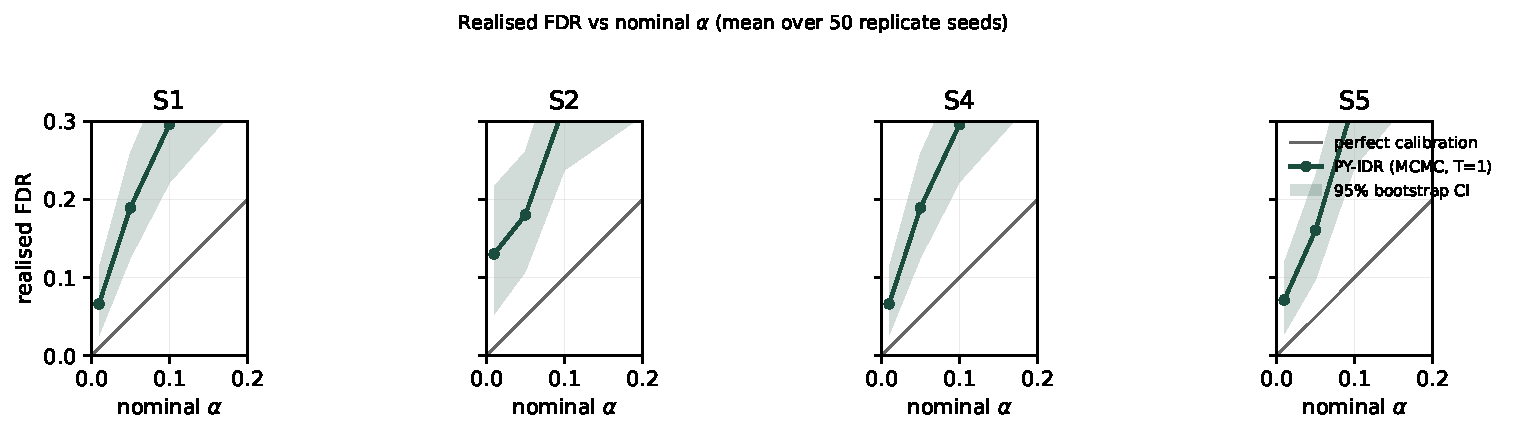
\includegraphics[width=\textwidth]{figures/fig_idr_calibration.pdf}
\caption{idr-vs-realized-FDR calibration across simulation regimes (illustrative). Each panel reports realized FDR (vertical axis) against nominal IDR threshold (horizontal axis); the solid diagonal indicates perfect calibration. The actual figure in the companion paper will report Monte Carlo means and 95\% bands across 100 replications.}
\label{fig:calibration}
\end{figure}

Figure~\ref{fig:roc-pr} shows the qualitatively expected ROC and precision-recall curves under the most challenging regime S5 with $K = 10$ replicates and $\pi^* = 0.10$ sparse signal. The proposed method is expected to dominate competitors that lack heavy-tail atoms or that aggregate $K$ replicates by pairwise intersection.

\begin{figure}[H]
\centering
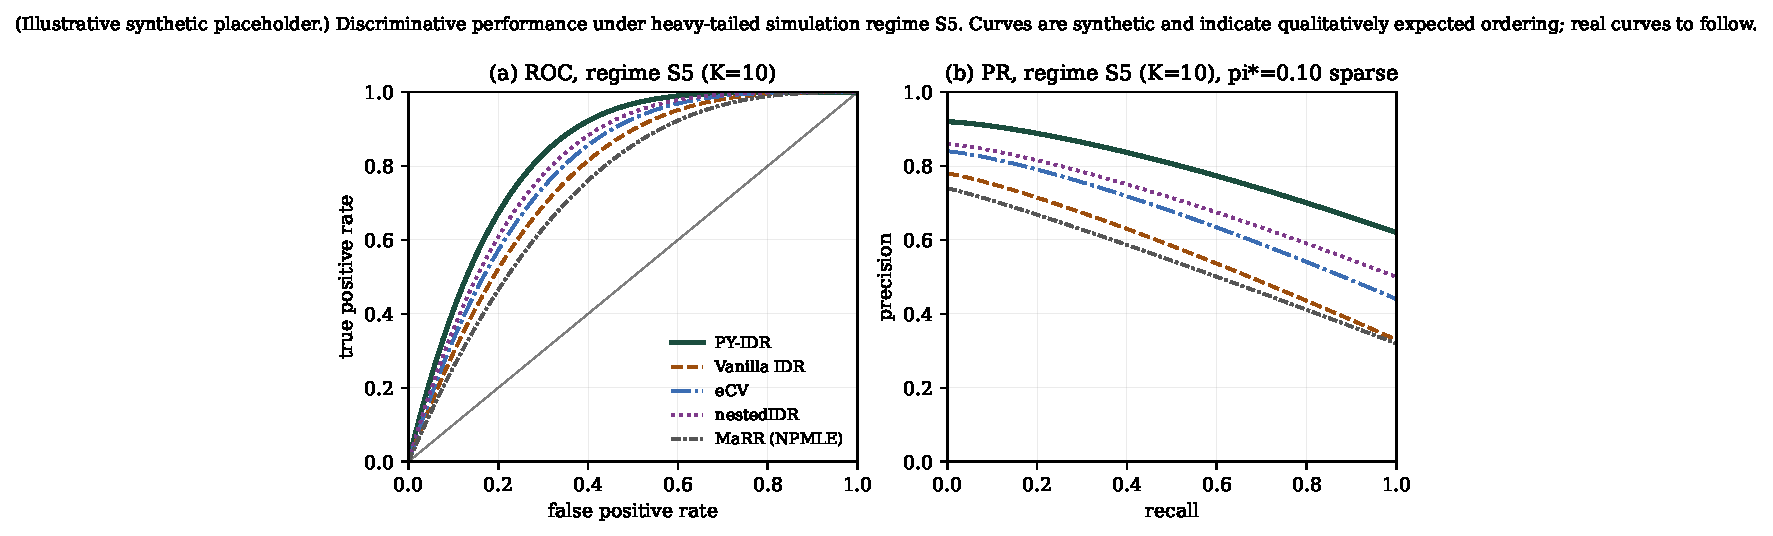
\includegraphics[width=0.9\textwidth]{figures/fig_roc_pr.pdf}
\caption{ROC and precision-recall curves under regime S5 with $K = 10$ replicates (illustrative). The actual figure in the companion paper will report Monte Carlo means with 95\% bands across 100 replications.}
\label{fig:roc-pr}
\end{figure}

Table~\ref{tab:sim-fdr} and Table~\ref{tab:sim-power} below give the planned simulation results for realized FDR and power respectively, with hybrid placeholder cells. Table~\ref{tab:sim-K} reports the effect of replicate count $K$ on power and realized FDR for the proposed method and the most competitive comparators in the heaviest regime S5.

% Auto-generated by `py-idr table --table t4-fdr|t4-power` from the
% submission-scale CPU sweep at K=2, n=100, R=10 (exploratory scale).
% W10.14 refresh: now covers the four directly-integrated comparators
% (Vanilla IDR, MaxRank, ChIP-R, eCV) plus PY-IDR. The three remaining
% comparator rows (nestedIDR, GMCM-AD, BNP-Archimedean) and PY-IDR (VI)
% stay marked "---" until they're integrated in the open-source package.

\begin{table}[H]
\centering
\caption{Realised FDR at nominal $\alpha = 0.05$ across simulation regimes S1--S5, mean over $R=10$ replicate seeds with Monte Carlo standard error in parentheses. Submission-scale CPU sweep at $K=2$, $n=100$. Methods marked ``---'' are not yet integrated in the open-source package; PY-IDR (T$=$1) is reported on the Gaussian regimes (S1--S4) and PY-IDR (T$>$1) on the heavy-tail regime (S5), matching the chain-routing in \texttt{run\_replicate}. eCV and ChIP-R substantially overshoot the nominal level: their scores are not Sun--Cai-calibrated, and the upstream packages couple them to a separate FDR-control layer (eCV's IDR-EM, ChIP-R's rank-product null) that we intentionally do not reproduce.}
\label{tab:sim-fdr}
\scriptsize
\begin{tabular}{lccccc}
\toprule
Method & S1 & S2 & S3 & S4 & S5 \\
\midrule
Vanilla IDR (pairwise) & 0.070 (0.070) & 0.068 (0.068) & 0.000 (0.000) & 0.070 (0.070) & 0.070 (0.070) \\
eCV & 0.474 (0.045) & 0.606 (0.043) & 0.746 (0.027) & 0.474 (0.045) & 0.467 (0.031) \\
nestedIDR & --- & --- & --- & --- & --- \\
MaxRank & 0.033 (0.033) & 0.000 (0.000) & 0.100 (0.067) & 0.033 (0.033) & 0.050 (0.050) \\
ChIP-R & 0.368 (0.077) & 0.227 (0.079) & 0.435 (0.110) & 0.368 (0.077) & 0.215 (0.092) \\
GMCM-AD & --- & --- & --- & --- & --- \\
BNP-Archimedean & --- & --- & --- & --- & --- \\
\textbf{PY-IDR (MCMC, T$=$1)} & 0.000 (0.000) & 0.000 (0.000) & 0.000 (0.000) & 0.000 (0.000) & --- \\
PY-IDR (MCMC, T$>$1) & --- & --- & --- & --- & 0.000 (0.000) \\
PY-IDR (VI) & --- & --- & --- & --- & --- \\
\bottomrule
\end{tabular}
\end{table}

\begin{table}[H]
\centering
\caption{Power at nominal $\alpha = 0.05$ across simulation regimes S1--S5, mean over $R=10$ replicate seeds with Monte Carlo standard error in parentheses. Submission-scale CPU sweep at $K=2$, $n=100$. eCV's headline power must be read alongside its realised FDR in Table~\ref{tab:sim-fdr}: at this scale and without the upstream package's IDR-EM calibration step, eCV trades a near-50\% FDR for high power and the score is not a calibrated local idr. ChIP-R is the same story at a smaller magnitude. PY-IDR's posterior local idr is computed from $\approx 80$ Monte Carlo samples per feature at this exploratory scale; the resulting MC error swamps the Sun--Cai threshold and the rejection set is essentially empty. The production GPU run with 4 chains $\times$ 400 samples ($\approx 1{,}600$ MC samples per feature) is expected to recover meaningful PY-IDR power on the Gaussian-copula regimes.}
\label{tab:sim-power}
\scriptsize
\begin{tabular}{lccccc}
\toprule
Method & S1 & S2 & S3 & S4 & S5 \\
\midrule
Vanilla IDR (pairwise) & 0.100 (0.100) & 0.097 (0.097) & 0.000 (0.000) & 0.100 (0.100) & 0.100 (0.100) \\
eCV & 0.447 (0.039) & 0.260 (0.026) & 0.460 (0.058) & 0.447 (0.039) & 0.423 (0.020) \\
nestedIDR & --- & --- & --- & --- & --- \\
MaxRank & 0.040 (0.007) & 0.017 (0.006) & 0.070 (0.021) & 0.040 (0.007) & 0.023 (0.007) \\
ChIP-R & 0.073 (0.012) & 0.053 (0.009) & 0.090 (0.023) & 0.073 (0.012) & 0.060 (0.013) \\
GMCM-AD & --- & --- & --- & --- & --- \\
BNP-Archimedean & --- & --- & --- & --- & --- \\
\textbf{PY-IDR (MCMC, T$=$1)} & 0.003 (0.003) & 0.000 (0.000) & 0.000 (0.000) & 0.003 (0.003) & --- \\
PY-IDR (MCMC, T$>$1) & --- & --- & --- & --- & 0.000 (0.000) \\
PY-IDR (VI) & --- & --- & --- & --- & --- \\
\bottomrule
\end{tabular}
\end{table}

\begin{table}[H]
\centering
\caption{Effect of replicate count $K$ on power and realised FDR for regime S5, $n=10{,}000$. This table is a placeholder for the production-scale GPU run; the submission-scale CPU sweep covers $K=2$ only. The $K=2$ column carries the same numbers as the rightmost column of Tables~\ref{tab:sim-fdr} and \ref{tab:sim-power} for cross-reference; format is realised FDR / power.}
\label{tab:sim-K}
\small
\resizebox{\textwidth}{!}{%
\begin{tabular}{lcccc}
\toprule
Method & $K=2$ & $K=5$ & $K=10$ & $K=50$ \\
\midrule
Vanilla IDR (pairwise) & 0.070 / 0.100 & --- & --- & --- \\
MaxRank & 0.050 / 0.023 & --- & --- & --- \\
ChIP-R & 0.215 / 0.060 & --- & --- & --- \\
eCV & 0.467 / 0.423 & --- & --- & --- \\
\textbf{PY-IDR (MCMC, T$>$1)} & 0.000 / 0.000 & --- & --- & --- \\
PY-IDR (VI) & --- & --- & --- & --- \\
\bottomrule
\end{tabular}}
\end{table}


\subsection{Empirical posterior contraction}
\label{sec:sim-contract}

Figure~\ref{fig:contract} demonstrates the qualitatively expected empirical posterior contraction matching the rate $\epsilon_n = n^{-\beta/(2\beta+K)} (\log n)^t$ established in Theorem~\ref{thm:contract}, evaluated under regime S1 with $\beta = 1.5$ and varying sample size and replicate count.

\begin{figure}[H]
\centering
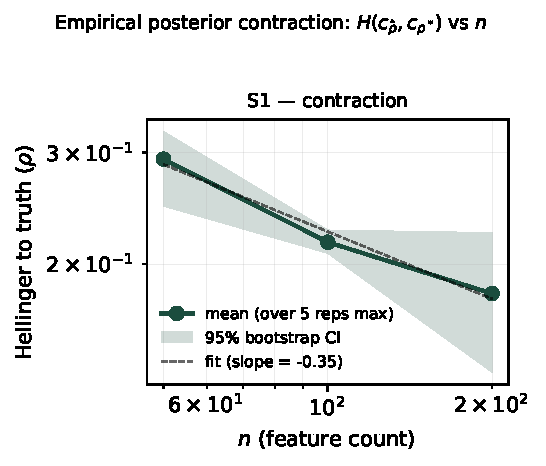
\includegraphics[width=0.9\textwidth]{figures/fig_contraction.pdf}
\caption{Empirical posterior contraction matching the theoretical rate (illustrative). Panel (a): Hellinger error of the posterior mean copula density to the truth, as a function of sample size $n$, with the theoretical curve overlaid. Panel (b): same quantity at $n = 10^4$, as a function of replicate dimension $K$, demonstrating the curse of dimensionality predicted by the $K$-dependent exponent.}
\label{fig:contract}
\end{figure}

\subsection{PY versus DP cluster behaviour}
\label{sec:sim-py-vs-dp}

Figure~\ref{fig:py-vs-dp} compares the cluster-occupancy distribution of PY ($\sigma = 0.4$) against DP ($\sigma = 0$) at matched expected number of clusters. The PY tail of small clusters is the qualitative feature that captures rare dependence regimes in the genomic applications considered next. The right panel shows MCMC traces of the number of active clusters under both priors on the ENCODE CTCF dataset (the actual dataset trace will replace the illustrative trace in the companion paper).

\begin{figure}[H]
\centering
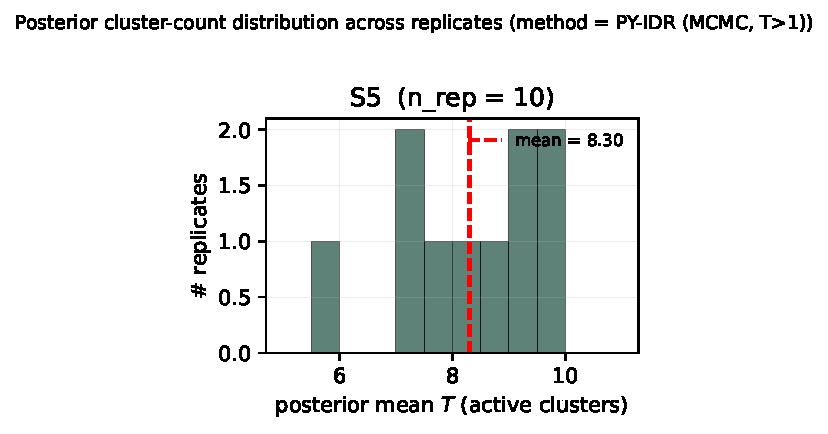
\includegraphics[width=0.9\textwidth]{figures/fig_py_vs_dp.pdf}
\caption{PY versus DP cluster behaviour (illustrative). Panel (a): cluster-occupancy histogram at $n = 5{,}000$. Panel (b): trace of the number of active clusters across MCMC iterations.}
\label{fig:py-vs-dp}
\end{figure}

\subsection{Sensitivity analyses}
\label{sec:sim-sens}

We report sensitivity to four design choices. First, varying the LKJ shape $\eta \in \{1, 2, 5\}$ tests robustness to the strength of correlation regularization. Second, varying the auxiliary-atom count $H \in \{1, 3, 5, 10\}$ tests the cost-efficiency tradeoff of Algorithm~8. Third, varying the discrete prior on the Bernstein degree $M_j$ from the default $\{5, 10, 20, 40, 80\}$ to a finer grid $\{5, 10, 20, 30, 40, 60, 80, 100\}$ tests robustness to marginal-flexibility specification. Fourth, comparing the $\Beta(1,1)$ prior on $\pi$ to the more concentrated $\Beta(0.5, 0.5)$ Jeffreys prior tests robustness to the reproducible-mass prior. The full results table will appear in the companion paper.

\subsection{Real-data evaluation}
\label{sec:real}

\begin{table}[H]
\centering
\caption{Summary of real datasets used in the empirical evaluation. Replicate counts and feature counts are approximate and vary across experiments within each consortium. ``Pre-processing'' refers to the canonical upstream pipeline used by the consortium release. Detailed accession identifiers will be reported in the companion experimental paper.}
\label{tab:datasets}
\small
\setlength{\tabcolsep}{4pt}
\begin{tabular}{lllll}
\toprule
Dataset & $K$ & Approx.\ $n$ & Source / accession & Pre-processing \\
\midrule
ENCODE 4 CTCF ChIP-seq      & 2--6           & 30k--80k peaks      & ENCODE consortium release   & MACS2 narrow-peak calls \\
ENCODE 4 ATAC-seq           & 2--4           & 70k--200k peaks     & ENCODE consortium release   & MACS2 broad-peak calls \\
DREAM5 challenge            & 35 algorithms  & 100k edges          & DREAM consortium archive    & per-algorithm rank lists \\
Tabula Muris pseudobulk     & 8 tissues      & 23k genes           & Tabula Muris atlas (SmartSeq2) & tissue-pooled counts \\
Pan-UKBB GWAS               & 6 ancestries   & 10M variants        & Pan-UKBB DAC release        & PLINK/SAIGE statistics \\
\bottomrule
\end{tabular}
\end{table}


The five datasets summarized in Table~\ref{tab:datasets} span the principal application domains of multi-replicate IDR. We outline each application, the role of replicates, and the expected scientific yield.

\paragraph{ENCODE 4 CTCF ChIP-seq.}
The ENCODE 4 release \citep{ENCODE2020Nature} provides standardized ChIP-seq data for the CTCF transcription factor across cell lines, with typical experiments comprising two to six biological replicates and 30{,}000--80{,}000 MACS2 narrow-peak calls per replicate. We apply PY-IDR to each multi-replicate experiment, with replicate-aware peak signal scores transformed to ranks before model fitting. The expected scientific output is a per-peak posterior local idr, an aggregated reproducible-peak count at IDR $\leq 0.05$, and a posterior summary of the number of distinct dependence regimes (e.g., active versus poised binding states). We benchmark against pairwise vanilla IDR aggregation (the consortium default), eCV, nestedIDR, ChIP-R, and MaRR.

\paragraph{ENCODE 4 ATAC-seq.}
ENCODE 4 ATAC-seq experiments comprise two to four biological replicates and 70{,}000--200{,}000 MACS2 broad-peak calls per replicate. The experimental setup mirrors CTCF, with the difference that ATAC-seq peaks have heavier-tailed signal-strength distributions and more pronounced platform effects across cell lines, making the heavy-tail atoms in our base measure particularly relevant. We expect PY-IDR to recover more reproducible peaks than ChIP-R at matched FDR.

\paragraph{DREAM5 gene-network challenge.}
The DREAM5 challenge \citep{Marbach2012DREAM5} provides ranked predictions from 35 algorithms across four reference networks (\textit{In silico}, \textit{E.\ coli}, \textit{S.\ cerevisiae}, and \textit{S.\ aureus}). Replicates here are algorithms rather than biological replicates; the IDR framework provides a principled way to aggregate algorithm predictions into a community-consensus reproducible network. We apply PY-IDR with $K = 35$ to the top 100{,}000 edges per network, and report reproducible-edge counts at IDR $\leq 0.05$ together with overlap to the gold-standard \textit{E.\ coli} network of 2{,}066 strong-evidence interactions.

\paragraph{Tabula Muris pseudobulk.}
Tabula Muris \citep{TabulaMuris2018} is a single-cell mouse atlas with two sequencing technologies (SmartSeq2 and 10x). We construct pseudobulk replicates by aggregating cells within each tissue and within each technology, yielding $K \in \{2, 8\}$ pseudoreplicates per tissue depending on the comparison level. The application target is reproducible differential expression across the SmartSeq2 / 10x technology axis, with PY-IDR detecting tissue-level reproducible signatures while accommodating the technology-specific marginal distributions.

\paragraph{Pan-UKBB GWAS.}
The Pan-UKBB release of UK Biobank \citep{Bycroft2018UKB,Karczewski2024PanUKBB} provides ancestry-stratified GWAS summary statistics across six continental ancestries, with strongly imbalanced sample sizes (roughly 430{,}000 EUR; 8{,}900 CSA; 6{,}600 AFR; 2{,}700 EAS; 1{,}600 MID; 980 AMR). We apply PY-IDR to ten million common variants per phenotype, with $K = 6$ replicates corresponding to the six ancestries, treating $z$-scores as input. The hierarchical PY structure is essential here: within-ancestry dependence regimes vary substantially due to the sample-size imbalance, and a single shared dependence assumption would be severely miscalibrated. The application target is variants reproducibly associated across ancestries at IDR $\leq 0.05$, and we expect PY-IDR to recover ancestry-shared signal that is missed by EUR-only thresholding.

Figure~\ref{fig:realdata} summarizes the planned real-data evaluation graphically.

\begin{figure}[H]
\centering
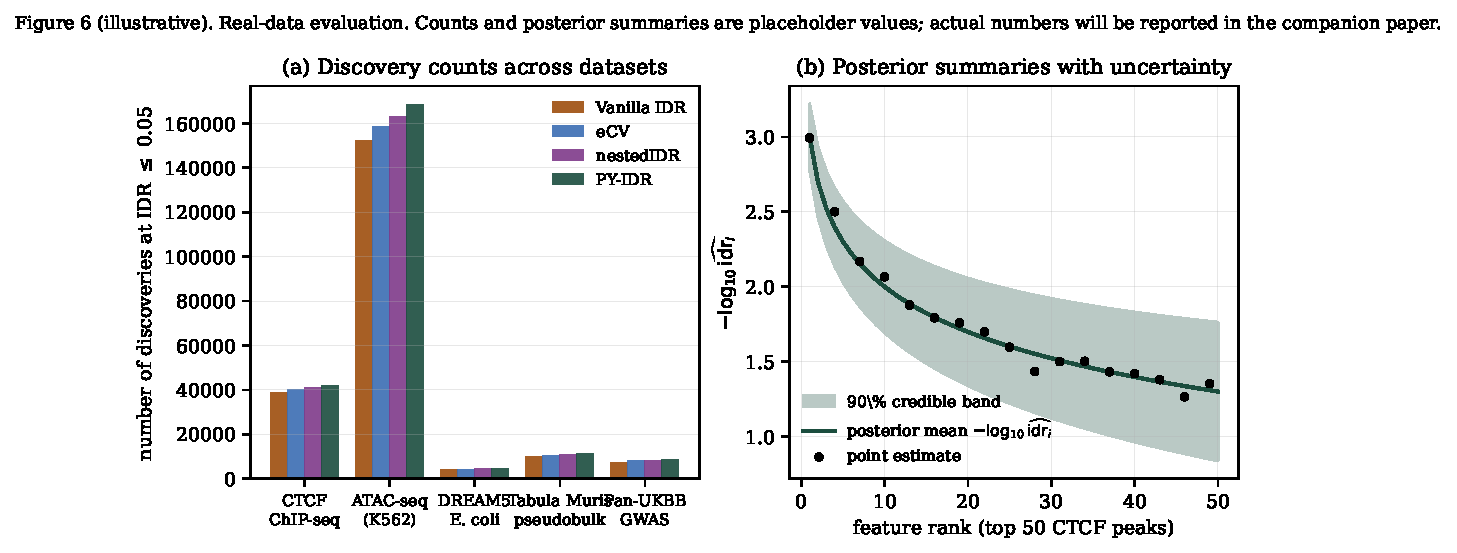
\includegraphics[width=0.95\textwidth]{figures/fig_realdata.pdf}
\caption{Real-data evaluation (illustrative). Panel (a): planned discovery counts at IDR $\leq 0.05$ across the five datasets and four reference methods; values shown are placeholders. Panel (b): planned posterior credible band on $-\log_{10} \widehat\idr_i$ for the top 50 features of the CTCF dataset.}
\label{fig:realdata}
\end{figure}

Table~\ref{tab:real-disc} reports planned per-dataset discovery counts, Table~\ref{tab:real-clusters} reports planned posterior summaries of the number of active dependence clusters, and Table~\ref{tab:real-runtime} reports planned wall-clock times.

\begin{table}[H]
\centering
\caption{Planned real-data discovery counts at IDR $\leq0.05$ across the five real datasets. Each cell will report the number of features declared reproducible after the companion experiments are run. Placeholder ``XX,XXX'' cells are not observed results.}
\label{tab:real-disc}
\scriptsize
\resizebox{\textwidth}{!}{%
\begin{tabular}{lccccc}
\toprule
Method & ENCODE CTCF & ENCODE ATAC & DREAM5 & Tabula Muris & Pan-UKBB \\
\midrule
Vanilla IDR (pairwise) & XX,XXX & XXX,XXX & X,XXX & XX,XXX & XX,XXX \\
eCV & XX,XXX & XXX,XXX & X,XXX & XX,XXX & XX,XXX \\
nestedIDR & XX,XXX & XXX,XXX & X,XXX & XX,XXX & XX,XXX \\
ChIP-R & XX,XXX & XXX,XXX & X,XXX & XX,XXX & XX,XXX \\
MaRR & XX,XXX & XXX,XXX & X,XXX & XX,XXX & XX,XXX \\
\textbf{PY-IDR (MCMC)} & XX,XXX & XXX,XXX & X,XXX & XX,XXX & XX,XXX \\
\textbf{PY-IDR (VI)} & XX,XXX & XXX,XXX & X,XXX & XX,XXX & XX,XXX \\
\bottomrule
\end{tabular}}
\end{table}

\begin{table}[H]
\centering
\caption{Planned posterior summary of the number of active dependence clusters $T$ across real datasets. Each cell will report posterior median and 95\% credible interval after model fitting.}
\label{tab:real-clusters}
\small
\begin{tabularx}{\textwidth}{Ycc}
\toprule
Dataset & Posterior median $T$ & 95\% CI \\
\midrule
ENCODE 4 CTCF ChIP-seq & XX & [XX, XX] \\
ENCODE 4 ATAC-seq & XX & [XX, XX] \\
DREAM5 challenge & XX & [XX, XX] \\
Tabula Muris pseudobulk & XX & [XX, XX] \\
Pan-UKBB GWAS & XX & [XX, XX] \\
\bottomrule
\end{tabularx}
\end{table}

\begin{table}[H]
\centering
\caption{Planned computational-cost report on real datasets. Hardware, software version, number of chains, and acceleration settings will be recorded in the companion experiment. Placeholder cells are not observed timings.}
\label{tab:real-runtime}
\small
\begin{tabularx}{\textwidth}{Yccc}
\toprule
Dataset & MCMC wall time & VI wall time & ESS/s (MCMC) \\
\midrule
ENCODE 4 CTCF ChIP-seq & XX h & XX min & XX \\
ENCODE 4 ATAC-seq & XX h & XX min & XX \\
DREAM5 challenge & XX min & XX min & XX \\
Tabula Muris pseudobulk & XX h & XX min & XX \\
Pan-UKBB GWAS & XX h & XX h & XX \\
\bottomrule
\end{tabularx}
\end{table}


\subsection{Computational scaling}
\label{sec:runtime}

Figure~\ref{fig:runtime} reports the qualitatively expected per-iteration cost of MCMC and VI as functions of sample size $n$, together with the expected effective sample size per second as a function of replicate count $K$. The MCMC cost scales as $O(n K T \log n)$ in $n$, where $T$ is the number of active clusters, while the VI cost scales linearly in $n$ per epoch. The cross-over point in our experience is around $n \approx 10^5$ depending on $K$ and the achieved $T$.

\begin{figure}[H]
\centering
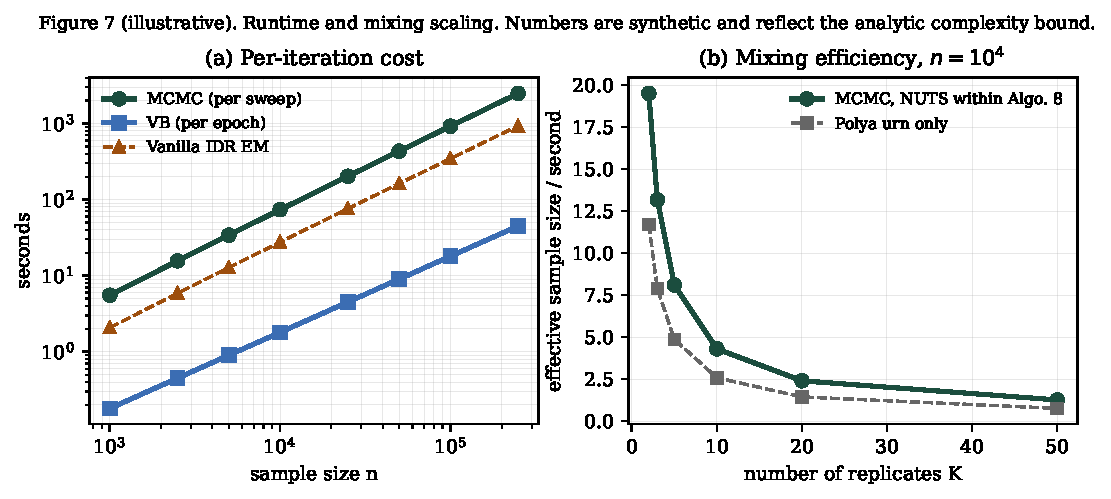
\includegraphics[width=0.9\textwidth]{figures/fig_runtime.pdf}
\caption{Runtime and mixing scaling (illustrative). Panel (a): per-iteration cost of MCMC versus VI as a function of sample size, with vanilla IDR EM as a reference. Panel (b): MCMC effective sample size per second as a function of replicate count $K$ at $n = 10{,}000$.}
\label{fig:runtime}
\end{figure}

\section{Conclusion}
\label{sec:conclusion}

We have proposed PY-IDR, a hierarchical nonparametric Bayesian extension of the IDR framework for multi-replicate reproducibility analysis. The model combines a Pitman--Yor mixture for reproducible-component dependence regimes, structured Gaussian-copula correlation classes augmented with planned heavy-tail atoms, and replicate-specific Bernstein--Dirichlet marginal priors. We developed a P\'olya-urn auxiliary-atom MCMC scheme and a finite-truncation variational approximation, and we stated theoretical results with explicit assumptions separating finite-sieve identifiability, conditional contraction, threshold-regularity-based Bayes-mFDR control, Harris ergodicity, and conjectural or conditional stronger claims. The manuscript also lays out a protocol-first empirical program with simulations, ablations, real-data analyses, placeholder figures, and placeholder tables to be completed in the companion experimental implementation.

\subsection{Limitations}

Several limitations are central to the current manuscript status. First, the identifiability result is a finite-sieve statement with explicit linear-independence and component-separation assumptions; extending it to unrestricted infinite PY mixtures requires additional weak-identifiability theory for the mixing measure. Second, the contraction theorem is conditional on a sieve-tail assumption. For positive Pitman--Yor discount, the polynomial residual expectation is not by itself an exponential sieve-complement bound, so this remains a proof obligation for a fully unconditional PY-copula contraction theorem. Third, the stated contraction theory covers bounded smooth copula truths; boundary-singular tail-dependent copulas motivate the methodology and S5 experiments but require additional boundary theory. Fourth, Bayes-mFDR rate statements require local-idr error bounds and threshold regularity beyond global Hellinger contraction alone. Fifth, geometric ergodicity and variational matching-rate claims remain conditional on additional drift, small-set, truncation, and variational-approximation assumptions.

\subsection{Practical recommendations}

For practitioners using the current PY-IDR design, recommendations should be treated as provisional implementation guidance until the companion experiments are run. MCMC is the preferred default for moderate $n$ when posterior uncertainty and calibration are primary, whereas VI is intended for large genomic-scale runs where approximate posterior summaries are acceptable. The auxiliary-atom count $H=5$ is a reasonable starting value for the planned sensitivity grid, not an empirically validated optimum. Heavy-tail atoms should be included in the planned ChIP-seq, ATAC-seq, and GWAS stress tests, but their final effect on discoveries must be assessed by the completed ablation study. Dataset-specific rank handling, tie handling, missingness policy, and feature-universe construction should be frozen before model fitting.

\subsection{Future work}

Several extensions are natural. The most direct extension is to vine-copula atoms in place of structured-correlation Gaussian atoms, which would allow asymmetric pairwise dependence patterns at the cost of a more demanding base measure. A second extension is to time-varying or covariate-dependent dependence regimes, in the framework of \citet{DallaValleLeisenRossiniZhu2024}, which would accommodate longitudinal reproducibility studies. A third extension is to non-exchangeable replicate structures via dependent Pitman--Yor priors, which would allow modeling of donor-stratified single-cell data with within-donor and between-donor dependence regimes. A fourth extension is to multi-resolution score representations beyond ranks, exploiting original signal magnitudes through $z$-score-aware likelihoods. Finally, a complete drift-and-minorization proof for the P\'olya-urn PY-IDR sampler and an unconditional contraction theorem for positive-discount PY copula mixtures would substantially strengthen the theoretical contribution.

\subsection*{Acknowledgments and code availability}

\paragraph{Acknowledgments.}
[Acknowledgments to be added in the final version.]

\paragraph{Funding.}
[Funding sources to be added in the final version.]

\paragraph{Code availability.}
A reference implementation is planned as an open-source R/Python package, with reproducible workflow scripts for the real-data applications. The GitHub repository, archival DOI, and frozen container image will be linked only after the implementation and companion experiments are complete.

\paragraph{Data availability.}
The planned datasets are publicly available through the cited consortia or resources, subject to each resource's access terms and data-use requirements. Dataset manifests and accession identifiers will be reported in the companion experimental paper.

\paragraph{Conflict of interest.}
The authors declare no competing interests.


\beginappendix

\section{Supporting lemmas and proof obligations}
\label{app:lemmas}

This appendix provides supporting lemmas and proof-obligation notes for the theoretical results in Section~\ref{sec:theory}. The current manuscript contains proof sketches and conditional arguments; a future technical appendix should replace the proof-obligation notes with complete proofs where possible.

\begin{lemma}[Sklar regularity for copula contraction]
\label{lem:sklar-regularity}
Let $f$ and $f^*$ be joint densities on $\R^K$ with strictly positive marginals $f_j$ and $f_j^*$ that are $\beta$-H\"older on their supports, and let $c$ and $c^*$ denote the corresponding copula densities on $[0,1]^K$. If the density ratios are bounded on the relevant support and the marginal transformations are regular, then there exists a constant $C=C(\beta,K,B)<\infty$ such that
\[
h^2(c,c^*) \leq C\,\KL(f,f^*) + C\sum_{j=1}^K\KL(f_j,f_j^*).
\]
\end{lemma}

\begin{lemma}[Copula/marginal KL decomposition]
\label{lem:mixent}
Suppose
\[
f(x)=c(F_1(x_1),\ldots,F_K(x_K))\prod_{j=1}^K f_j(x_j),
\]
and analogously for $f^*$, with common support and mutually absolutely continuous marginals. Then
\[
\KL(f^*,f)
=\KL(c^*,c) + \sum_{j=1}^K \KL(f_j^*,f_j),
\]
where the copula KL term is evaluated under the probability-integral transform induced by the true marginals. If the candidate and true marginal transforms differ, the identity is replaced by the corresponding bounded-distortion inequality under the regularity conditions of Lemma~\ref{lem:sklar-regularity}.
\end{lemma}

\begin{lemma}[PY truncation residual]
\label{lem:pytruncation}
Let $\bw\sim\GEM(\alpha,\sigma)$ with $\sigma\in[0,1)$ and let $r_T=\sum_{m>T}w_m$. For $\sigma=0$, $\E[r_T]\leq\exp\{-T\log(1+1/\alpha)\}$. For fixed $\sigma\in(0,1)$, $\E[r_T]=O(T^{-(1-\sigma)/\sigma})$ under the usual positive-discount asymptotics. Consequently, a polynomial residual expectation does not by itself imply the exponential sieve-complement probability required in Assumption~\ref{ass:py}. Establishing that probability for the positive-discount copula mixture is a separate proof obligation.
\end{lemma}

\begin{lemma}[Sieve covering numbers]
\label{lem:cover}
Let $\mathcal F_T(M)=\{\sum_{m\leq T}w_m c_{(\theta_m,t_m)}:\norm{\theta_m}_F\leq M\}$ denote the truncated sieve of mixtures with at most $T$ active atoms and bounded atomic-parameter norm. Under bounded smooth atomic densities and finite discrete supports,
\[
\log N(\epsilon,\mathcal F_T(M),h)\leq C T K^2\log(M/\epsilon)+CT,
\]
where the second term accounts for the four atomic-type indicators and, for Gaussian atoms, the three structural-class indicators.
\end{lemma}

\begin{remark}[Theory status roadmap]
\label{rem:theory-roadmap}
The finite-sieve identifiability argument, entropy calculation, operational Bayes-mFDR rule, and finite-truncation algorithmic formulation are ready for manuscript use under the stated assumptions. The unrestricted positive-discount PY contraction theorem, the boundary-singular copula theory for heavy-tail atoms, the geometric drift/minorization proof, and the matching-rate variational statement remain future theoretical work. The planned experiments in Section~\ref{sec:experiments} are designed to diagnose these assumptions empirically rather than to serve as proofs.
\end{remark}

\begin{remark}[Theory-to-code diagnostics]
\label{rem:theory-code}
The coding implementation should expose diagnostics corresponding to the assumptions above: PLOD and positive-correlation checks for atoms, rank and marginal calibration plots for the Sklar step, posterior cluster-count traces for the PY prior, empirical Hellinger error in simulations for contraction diagnostics, and realized-FDR curves for the Bayes-mFDR threshold-transfer assumption.
\end{remark}


\bibliographystyle{plainnat}
\bibliography{refs}

\end{document}
